\documentclass[10pt]{article}
\usepackage[margin=1in]{geometry}
\usepackage{blindtext}
\usepackage{graphicx}
\usepackage{subfig}
\usepackage{verbatim}
\graphicspath{ {./images/}   }

\begin{document}

\title{\textbf{ECSE 324 Computer Organization}\\
    Laboratory 2\\
    I/O
}

\author{Seyed Yazdan Zinati}
\maketitle

\begin{abstract}
    In this laboratory, we implement drivers for I/O devices of the DE1-SoC computer in ARM assembly. These drivers include drivers for slider switches, LEDs, HEX displays, pushbuttons, and timers. We then use the mentioned drivers to write different programs; namely, we program stopwatches using polling and interrupts. Through these programs, we exercise our understanding of memory-mapped I/O, polling, and interrupts.
\end{abstract}

\section{Basic I/O}
In this section, we implement drivers for slider switches, LEDs, HEX displays, and pushbuttons.
\subsubsection*{Slider switches and LEDs}
We use memory-mapped I/O to implement drivers to read from the slider switches and write to LEDs. The \verb+read_slider_switches_ASM+ subroutine reads from the slider switch data register and stores it into \verb+R0+.  On the other hand, the\verb+ write_LEDs_ASM+ subroutine stores the value in \verb+R0+ into the LED data register. Both subroutines are similar as they save used registers onto the stack, load the data register addresses, read or write to them using word accesses, and branch back to the callee. As both use one-hot encoding, calling them sequentially will turn on LEDs corresponding to the state of the switches. We name this subroutine \verb+switch_to_LED+.
\subsubsection*{HEX displays}
We implement three drivers for the HEX displays. The three drivers receive display indices to write into through \verb+R0+. \verb+HEX_clear_ASM+ turns off while \verb+HEX_flood_ASM+ turns all the segments of of the HEX displays. \verb+HEX_write_ASM+ receives an additional argument through \verb+R1+ indicating the HEX digit to display.

All three subroutines follow the same order. First, the display code to be written to the HEX display is determined. To do so, we load the display codes corresponding to hexadecimal digits with an immediate offset as they are stores as a byte array in consecutive memory locations. For instance, \verb+LDRB R2, [R3, #5]+ where \verb+R3+ is the byte array base address loads the display code corresponding to 5 into \verb+R2+.

Then, we enter a loop that checks which displays were passed as arguments and writes to them. We keep track of the display index with a loop counter that starts from zero, and we perform a \verb+TST+ logical test to determine if the encoding bit corresponding to a display is on. At the end of our loop, we increment the loop counter and perform a logical shift left on the register used to perform the \verb+TST+ operation to check for the next display. Each time we encounter a display passed as an argument in our loop, we write to it by finding the corresponding data register base address and offset.

The main challenge in writing the HEX display drivers was understanding one-hot encoding and ensuring code conciseness and readability. We achieved a concise code using a byte array to find display codes instead of checking for all 16 values, a loop to find the displays to write to, and automatically finding the base address and offset for each display.
\subsubsection*{Push buttons}
In this part, we write seven subroutines for pushbuttons. However, unlike LEDs, HEX displays, and slider switches, pushbuttons have interrupt mask and edge capture registers in addition to a data register.

Pushbutton read and write subroutines such as \verb+read_PB_data_ASM+, \verb+read_PB_edgecp_ASM+, and \verb+PB_clear-+ \verb+_edgecp_ASM+ operate in a similar way to the previously described LED write and slider switch read subroutines. The two \verb+PB_edgecp_is_pressed_ASM+ and \verb+PB_data_is_pressed_ASM+ subroutines perform an \verb+AND+ operation between the subroutine argument and the return value of \verb+read_PB_edgecp_ASM+ and \verb+read_PB_data_ASM+ respectively. To enable and disable interrupts for the corresponding pushbuttons in \verb+enable_PB_INT_ASM+ and \verb+disable_PB_INT_ASM+, we update the interrupt mask register with the result of \verb+ORR+ and \verb+BitClear+ operations between the subroutine input and the interrupt mask register respectively.

The main challenge faced in this part was manipulating bits using decscribed logical operations.
\subsubsection*{Simple I/O application}
To test the drivers we wrote so far, we write an application that maps slider switched directly to LEDs, floods \verb+HEX4+ and \verb+HEX5+ displays, and displays the value set using slider switches \verb+SW0-SW3+ on the HEX displays corresponding to the pressed pushbuttons. Additionally, \verb+SW9+ clears all HEX displays.

This program executes in an infinite loop. We first call the previously described \verb+switch_to_LED+ subroutine. Then, we flood \verb+HEX4+ and \verb+HEX5+ displays by calling \verb+HEX_flood_ASM+ with the argument being the one-hot encoding for \verb+HEX4+ and \verb+HEX5+ displays. Next, we isolate \verb+SW0-SW3+ and \verb+SW9+ switches using an \verb+AND+ operation. We check if the \verb+SW9+ bit is on and call \verb+HEX_clear_ASM+ with \verb+HEX0+ to \verb+HEX3+ displays as arguments if the condition is true. Finally, we call the \verb+HEX_write_ASM+ subroutine by passing the pushbuttons and \verb+SW0-SW3+ switches as the display indices (\verb+R0+) and hexadecimal digit to display (\verb+R1+) respectively.

\section{Timers}
In this section, we write drivers for the ARM A9 private timer and use it to implement an up counter and a stopwatch that use polling.

We interact with three of the four registers of the ARM A9 private timer: the load, control, and interrupt status registers. The \verb+ARM_TIM_config_ASM+ subroutine receives two arguments. The first argument is the initial count that we write into the load register of the timer. The second argument is the control bits (IAE bits) and prescaler value which we write into the control registers. \verb+ARM_TIM_read_INT_ASM+ and \verb+ARM_TIM_clear_INT_ASM simply+ read and clear the interrupt status register similar to previously described drivers.

\subsubsection*{Up counter}
We implement an up counter that counts in increments of one second from 0 to 15 and displays it on the HEX0 display. The timer restarts when the value 15 is reached. The application flowchart is illustrated in Figure 1.

The ARM A9 private timer uses a clock frequency of 200Mhz. Therefore, to count in increments of 1 second, we use an initial count of 200'000'000.   Moreover, we want to start the timer and automatically load the initial count when the timer reaches zero. To achieve this, we set both \verb+A+ and \verb+E+ bits in the control register to 1. We call the previously implemented \verb+ARM_TIM_config_ASM+ to configure the timer.

Next, we initialize a counter variable to zero and enter the polling loop. Inside the loop, we display the counter value into the \verb+HEX0+ display by calling \verb+HEX_write_ASM+ and poll the \verb+F+ bit of the interrupt status register to determine if the timer has reached zero. If the timer has not yet reached zero, we continue the loop. Otherwise, the counter gets incremented or set back to zero if the maximum count (15) has been reached, and the \verb+F+ bit is cleared by calling the \verb+ARM_TIM_clear_INT_ASM+ subroutine before branching to the polling loop.

\begin{figure}[h]
    \centering
    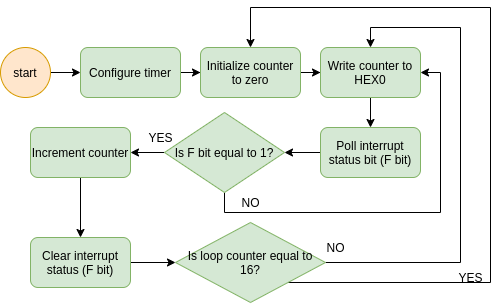
\includegraphics[scale=0.5]{diagram1}
    \caption{Up counter application flowchart}
\end{figure}
\subsubsection*{Polling-based stopwatch}
The polling-based stopwatch counts in increments of 10ms and uses PB0, PB1, and PB2 to start, stop, and reset the timer respectively. HEX0-1 display milliseconds, HEX2-3 display seconds, and HEX4-5 display minutes. Figure 2 shows the flowchart of the polling-based stopwatch.

\begin{figure}[h]
    \centering
    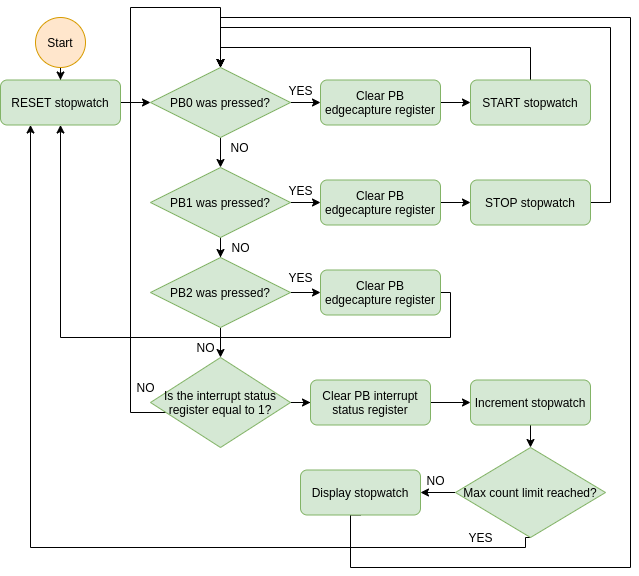
\includegraphics[scale=0.4]{diagram2}
    \caption{Stopwatch application flowchart}
\end{figure}

Similar to the simple up counter program, we use counters to keep track of time with the difference that we associate one counter to each hexadecimal display. For example, counter registers \verb+R3, R4, R5, R6, R7, R8+ keep track of centiseconds, deciseconds, seconds, decaseconds, minutes, and decaminutes respectively. Similar to the up counter, the application runs in a polling loop where we call the start, stop, and reset subroutines if their corresponding pushbuttons have been pushed and released by polling the pushbutton edge capture register using the \verb+PB_edgecp_is_pressed_ASM+ subroutine. The reset function simply sets all counter registers to zero, while the start and stop procedures configure the timer, by setting the \verb+E+ bit of the control register to 1 to start the timer and to 0 to stop it. As the timer runs at a clock frequency of 200MHz, we set the initial count to 2'000'000 to keep track of time with a precision of 10 milliseconds. We also poll the F bit of the timer interrupt status register and increment the counter value by 1 and write to the HEX displays if the \verb+F+ bit is equal to 1 (meaning that 10ms have passed). We also clear both polled registers if they contains a value other than zeros.

Incrementing the counters is different from the up-counter described in the previous section. We increment the value of the centisecond register by 1. However, if the value passes 9 after incrementing, we set the centiseconds register to 0 and increment the deciseconds register by 1 and continue this operation for all counter register. This process is slightly different for the decaseconds and the decaminute registers as a minute are 60 seconds, and an hour is 60 minutes. If the value passes 60 minutes (the maximum we can display), we reset the timer. We then write each counter register to their corresponding HEX display using \verb+HEX_write_ASM+.

\section{Interrupts}
\subsubsection*{Interrupt-based stopwatch}

\end{document}
